\documentclass[paper=letter,11pt]{scrartcl}

\KOMAoptions{headinclude=true, footinclude=false}
\KOMAoptions{DIV=14, BCOR=5mm}
\KOMAoptions{numbers=noendperiod}
\KOMAoptions{parskip=half}
\addtokomafont{disposition}{\rmfamily}
\addtokomafont{part}{\LARGE}
\addtokomafont{descriptionlabel}{\rmfamily}
%\setkomafont{pageheadfoot}{\normalsize\sffamily}
\setkomafont{pagehead}{\normalsize\rmfamily}
%\setkomafont{publishers}{\normalsize\rmfamily}
\setkomafont{caption}{\normalfont\small}
\setcapindent{0pt}
\deffootnote[1em]{1em}{1em}{\textsuperscript{\thefootnotemark}\ }


\usepackage{amsmath}
\usepackage[varg]{txfonts}
\usepackage[T1]{fontenc}
\usepackage{graphicx}
\usepackage{xcolor}
\usepackage[american]{babel}
% hyperref is needed in many places, so include it here
\usepackage{hyperref}

\usepackage{xspace}
\usepackage{multirow}
\usepackage{float}


\usepackage{braket}
\usepackage{bbm}
\usepackage{relsize}
\usepackage{tcolorbox}

\def\ketY{\ensuremath{\ket {\Psi}}}
\def\iGeV{\ensuremath{\textrm{GeV}^{-1}}}
%\def\mp{\ensuremath{m_{\textrm{proton}}}}
\def\rp{\ensuremath{r_{\textrm{proton}}}}
\def\me{\ensuremath{m_{\textrm{electron}}}}
\def\aG{\ensuremath{\alpha_G}}
\def\rAtom{\ensuremath{r_{\textrm{atom}}}}
\def\rNucl{\ensuremath{r_{\textrm{nucleus}}}}
\def\GN{\ensuremath{\textrm{G}_\textrm{N}}}
\def\ketX{\ensuremath{\ket{\vec{x}}}}
\def\ve{\ensuremath{\vec{\epsilon}}}


\def\ABCDMatrix{\ensuremath{\begin{pmatrix} A &  B  \\ C  & D \end{pmatrix}}}
\def\xyprime{\ensuremath{\begin{pmatrix} x' \\ y' \end{pmatrix}}}
\def\xyprimeT{\ensuremath{\begin{pmatrix} x' &  y' \end{pmatrix}}}
\def\xy{\ensuremath{\begin{pmatrix} x \\ y \end{pmatrix}}}
\def\xyT{\ensuremath{\begin{pmatrix} x & y \end{pmatrix}}}

\def\IMatrix{\ensuremath{\begin{pmatrix} 0 &  1  \\ -1  & 0 \end{pmatrix}}}
\def\IBoostMatrix{\ensuremath{\begin{pmatrix} 0 &  1  \\ 1  & 0 \end{pmatrix}}}
\def\JThree{\ensuremath{\begin{pmatrix}    0 & -i & 0  \\ i & 0  & 0 \\ 0 & 0 & 0 \end{pmatrix}}} 
\def\JTwo{\ensuremath{\begin{bmatrix}    0 & 0 & -i  \\ 0 & 0  & 0 \\ i & 0 & 0 \end{bmatrix}}}
\def\JOne{\ensuremath{\begin{bmatrix}    0 & 0 & 0  \\ 0 & 0  & -i \\ 0 & i & 0 \end{bmatrix}}}
\def\etamn{\ensuremath{\eta_{\mu\nu}}}
\def\Lmn{\ensuremath{\Lambda^\mu_\nu}}
\def\dmn{\ensuremath{\delta^\mu_\nu}}
\def\wmn{\ensuremath{\omega^\mu_\nu}}
\def\be{\begin{equation*}}
\def\ee{\end{equation*}}
\def\bea{\begin{eqnarray*}}
\def\eea{\end{eqnarray*}}
\def\bi{\begin{itemize}}
\def\ei{\end{itemize}}
\def\fmn{\ensuremath{F_{\mu\nu}}}
\def\fMN{\ensuremath{F^{\mu\nu}}}
\def\bc{\begin{center}}
\def\ec{\end{center}}
\def\nus{$\nu$s}

\def\adagger{\ensuremath{a_{p\sigma}^\dagger}}
\def\lineacross{\noindent\rule{\textwidth}{1pt}}

\newcommand{\multiline}[1] {
\begin{tabular} {|l}
#1
\end{tabular}
}

\newcommand{\multilineNoLine}[1] {
\begin{tabular} {l}
#1
\end{tabular}
}



\newcommand{\lineTwo}[2] {
\begin{tabular} {|l}
#1 \\
#2
\end{tabular}
}

\newcommand{\rmt}[1] {
\textrm{#1}
}


%
% Units
%
\def\m{\ensuremath{\rmt{m}}}
\def\GeV{\ensuremath{\rmt{GeV}}}
\def\pt{\ensuremath{p_\rmt{T}}}


\def\parity{\ensuremath{\mathcal{P}}}

\usepackage{cancel}
\usepackage{ mathrsfs }
\def\bigL{\ensuremath{\mathscr{L}}}

\usepackage{ dsfont }



\usepackage{fancyhdr}
\fancyhf{}


\lhead{\Large 33-444} % \hfill Introduction to Particle Physics \hfill Spring 2020}
\chead{\Large Introduction to Particle Physics} % \hfill Spring 2020}
\rhead{\Large Spring 2020} % \hfill Introduction to Particle Physics \hfill Spring 2020}

\begin{document}
\thispagestyle{fancy}

\begin{center}
{\huge \textbf{Lecture 26}}
\end{center}

{\fontsize{14}{16}\selectfont

\underline{\underline{Parity Violation}} 

This is an example of a little detail that did not look as expected and lead down a rabbit hole (only really resolved at the LHC) 


\underline{1950s}

Parity conservation is the idea that physics is unchanged if L and R are reversed. 

(eg: cant tell if your looking in a mirror or not)

What was found in the 50s was that some particle interactions distinguished L and R. 

\textbf{SHOCKING} could never happen in Gravity / EM or the strong force. 
(Was not tested in the weak interaction, b/c its weak its hard to study, but parity was assumed to hold there)

The weak interaction completely changed our ideas about what a force could be.


\be
\multilineNoLine{Observation of \\ Parity Violation }  \underbrace{\rightarrow}_{\rmt{Enrico Fermi}} \multilineNoLine{``V-A'' \\ theory} \underbrace{\rightarrow}_{\rmt{Precise, not fundamental}} \multilineNoLine{Weak \\ force}
\ee


Next few lecture we will explore this new force, lead us down a path with surprise after surprise, ultimately to the Higgs boson which provides a framework on which all of this sits. 


\lineacross

\clearpage

\underline{Discrete Lorentz Transformations}

Early in the course we discussed LT.

Focus was on continuous LT.  

Also discrete transformations that leave $t^2 - x^2$  invariant.

\underline{Parity}

\be
\parity\vec{x} = -\vec{x}
\ee

Can be thought of as viewing something in the mirror.

Vectors, like position and velocity are flipped by \parity.

\be
\parity \vec{v} = -\vec{v}
\ee

\be
\parity \left( \frac{dx}{dt} \right) = \frac{-1}{+1}
\ee

Other mathematical objects that transform as vectors under continuous LTs, but do not pick up a ``-'' sign under \parity.

``Pseudo-vectors'' (vampire vectors)

(Tend to arise from cross products.)

Example Angular Momentum  (torque and B-fields are others)

\be
\vec{L} = \vec{x} \times \vec{p} 
\ee

\bea
\parity(\vec{L}) &=& \parity(\vec{x}) \times \parity(\vec{p}) \\
 &=& -\vec{x} \times -\vec{p} = \vec{L}
\eea

\underline{Aside} Also notion of Scalars and Pseudo-scalars

\bc
\parity n = +n (scalars) or -n (pseudo-scalars) 
\ec

Maxwell's equations are invariant under \parity (Homework)

QCD and Gravity are also invariant.


\underline{Other discrete Lorentz Transforms}
\bi
\item[-] $\mathcal{T}$ - time reversal $\mathcal{T} t = -t $
\item[-] $\mathcal{C}$ - charge conjugation $\mathcal{C} q = -q $
\ei

Maxwell's equations invariant under $\mathcal{C}$ and $\mathcal{T}$ (also in HW)

Turns out that $\mathcal{T}$ needs to be defined as $\mathcal{T}i = -i$  to leave the Schrodinger equation invariant (more HW)

\lineacross

\underline{Parity Violation}

\bc
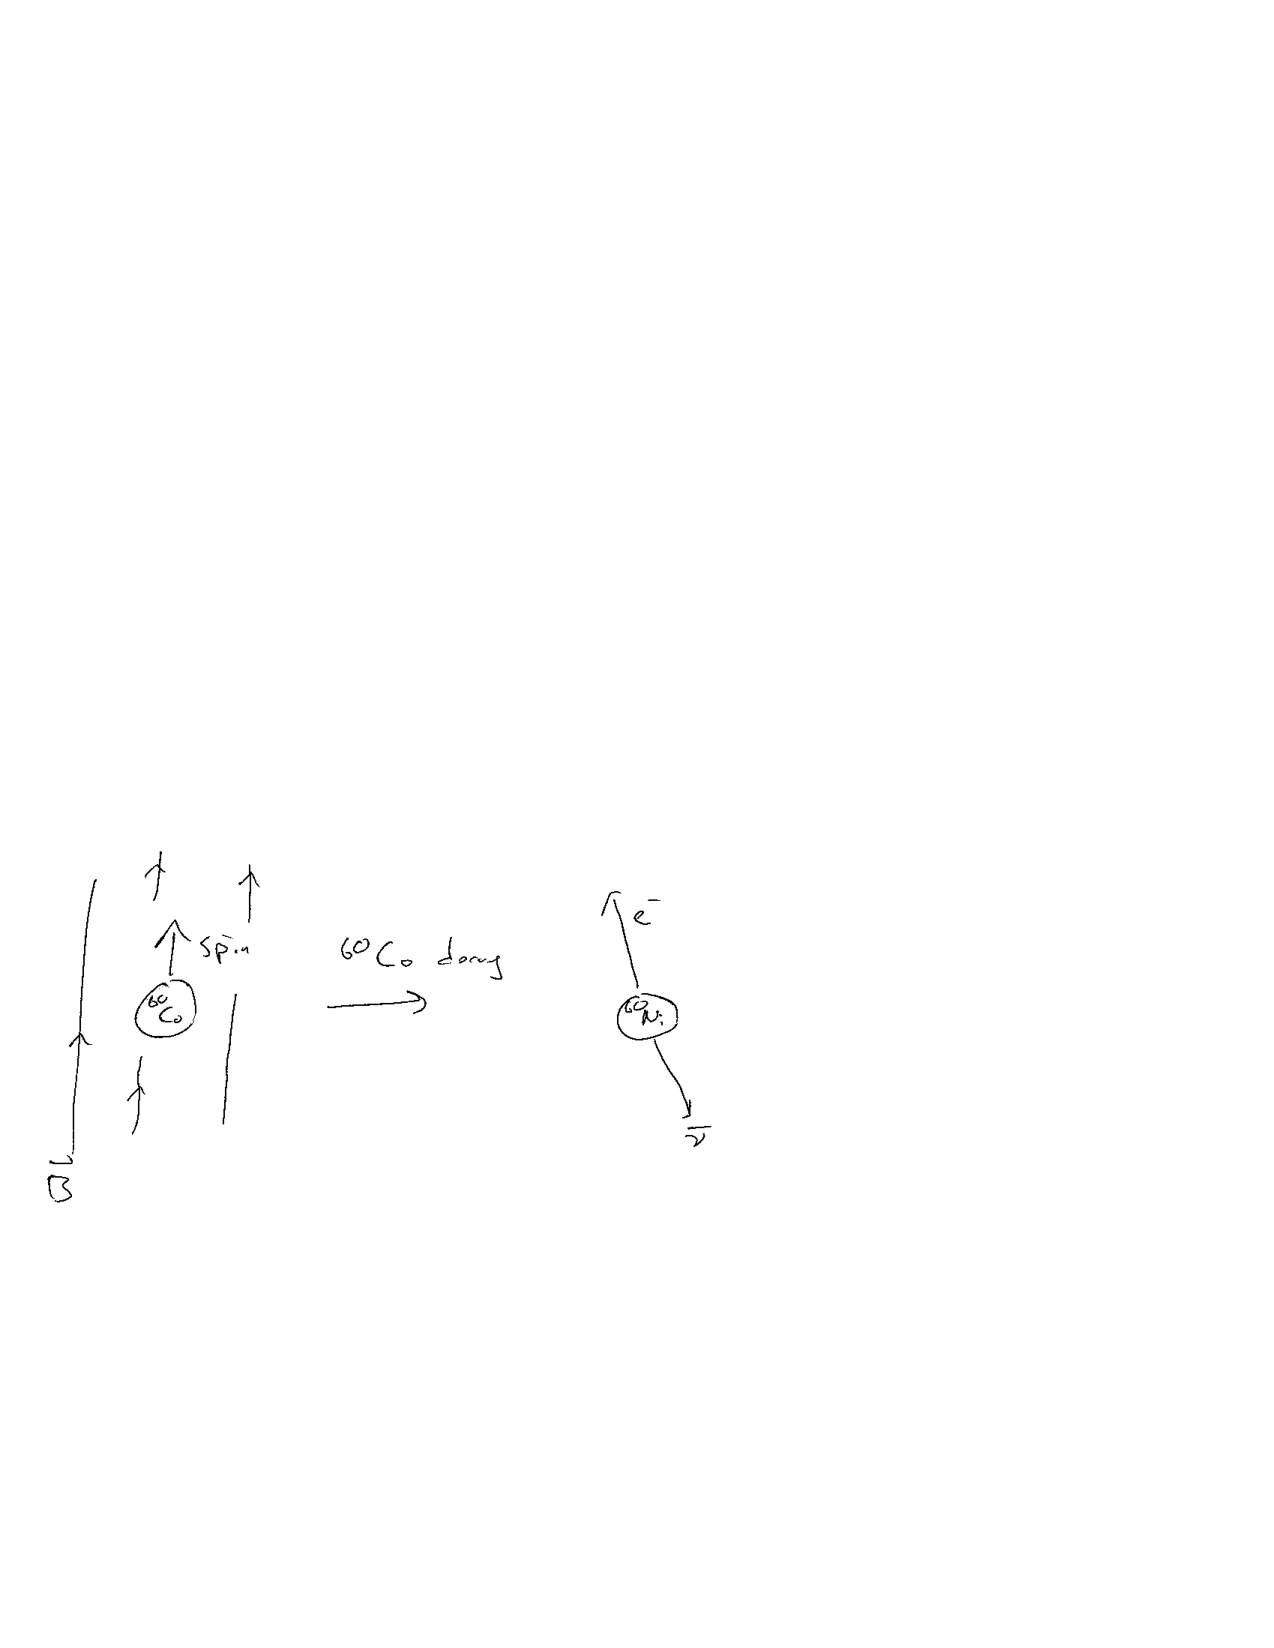
\includegraphics[width=0.725\textwidth]{./CobaltDecay.pdf}
\ec

\underline{Initial State}:  Invariant under \parity

\underline{Final State}:  

\bc
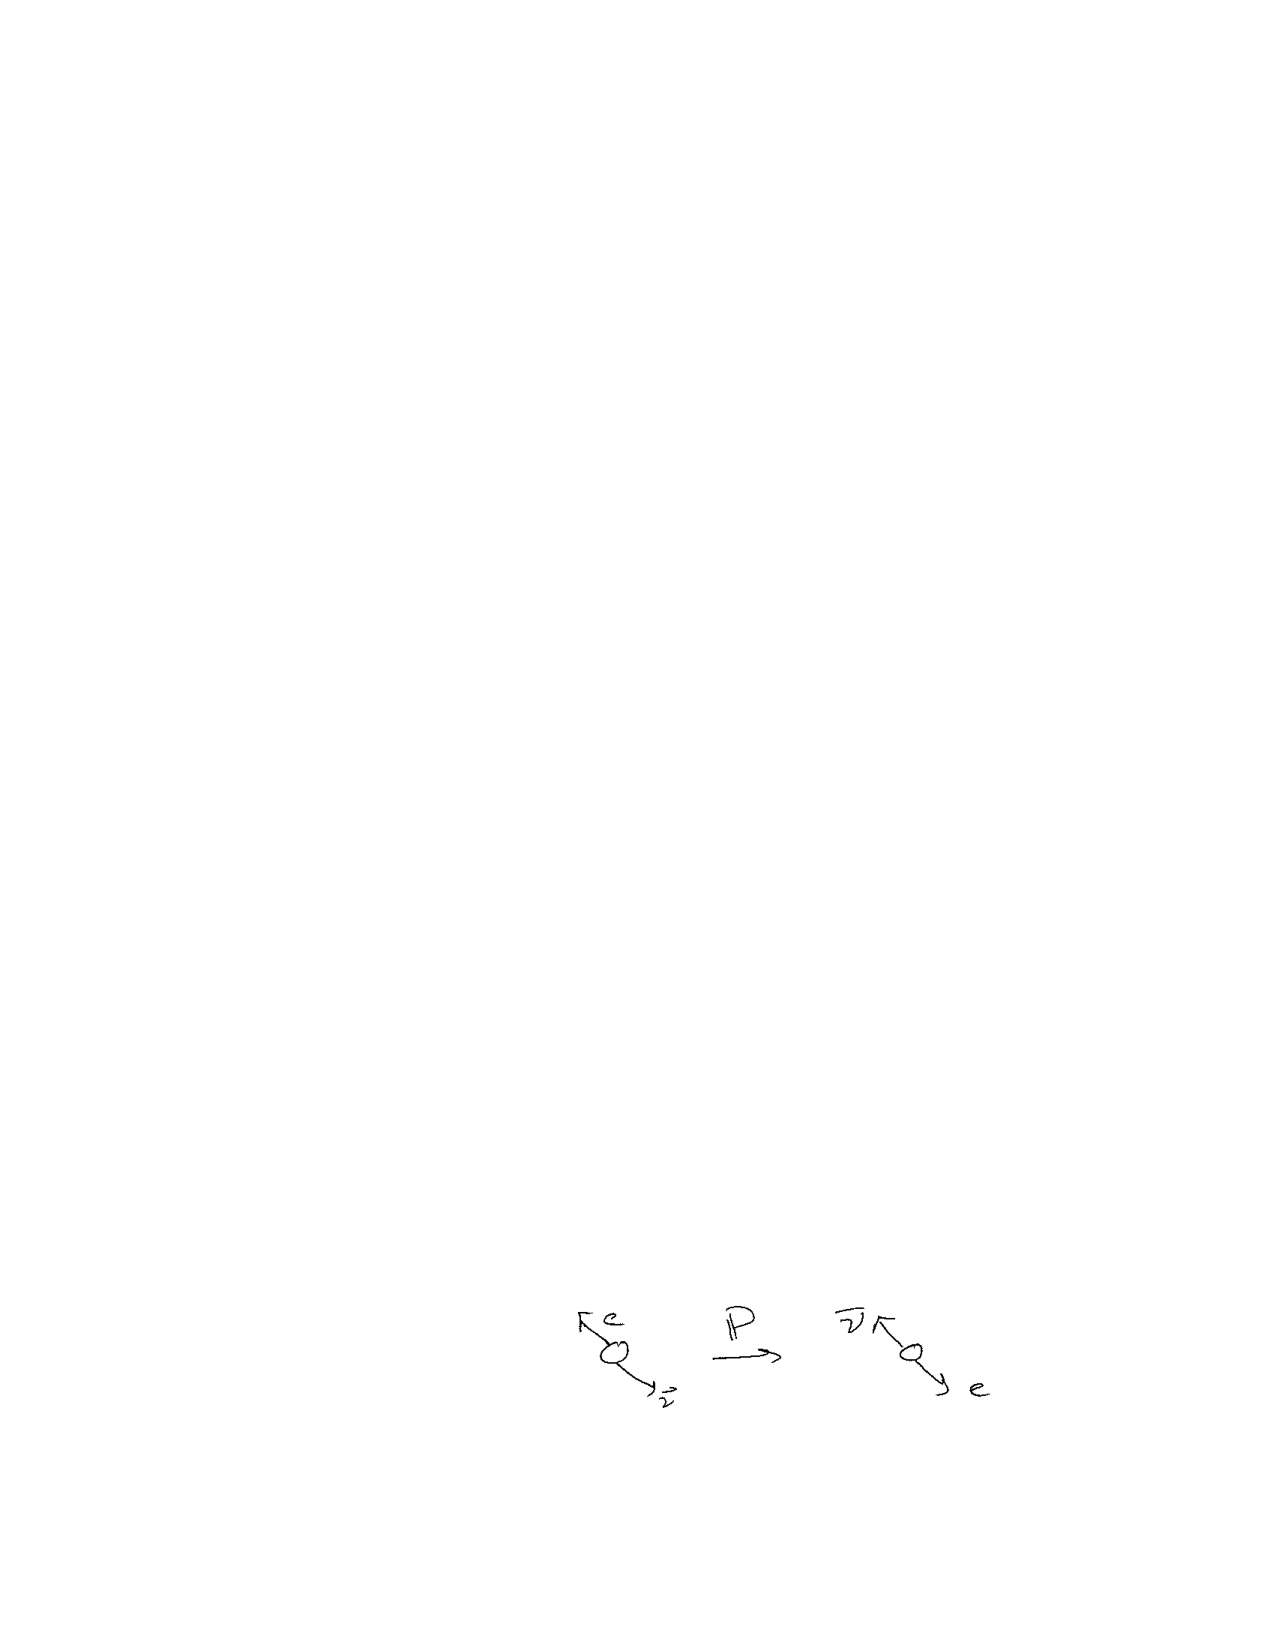
\includegraphics[width=0.5\textwidth]{./ParityOfCobaltDecay.pdf}
\ec

So under \parity\ the experimental setup is unchanged but the final configuration is flipped.
So if \parity\ is conserved, you should see both final configurations with equal probabilities.


Shocking result (due to C.S. Wu) more electrons emitted opposite to the direction of the spin. 

$\Rightarrow$ Force that governs nuclear decays violates parity!

\underline{Now} electron under parity changes handedness

\bc
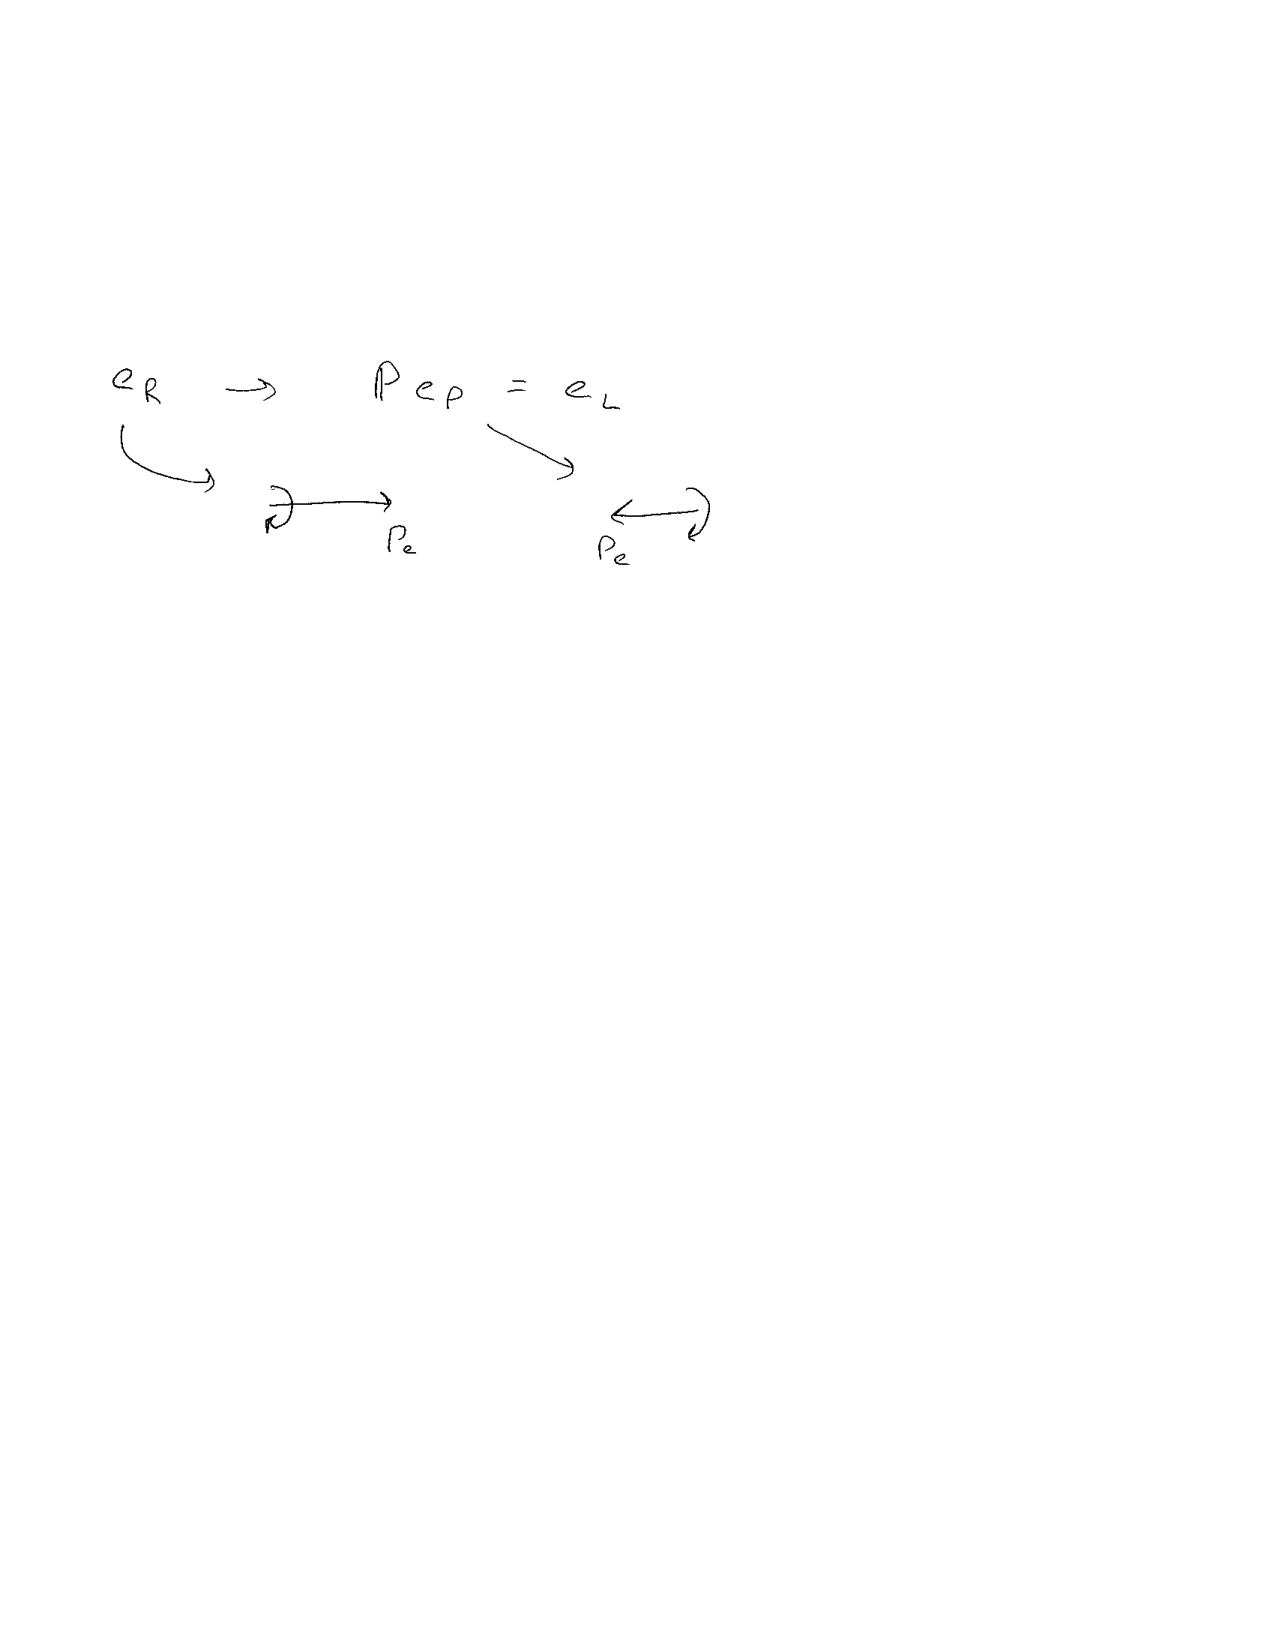
\includegraphics[width=0.5\textwidth]{./ElectronUnderPartity.pdf}
\ec


If parity violated by the nuclear (weak) interaction, we would expect different numbers of $e_R$ and $e_L$ produced in the $^{60}$Co decays.


In fact experiments showed that the produced electrons are \underline{Always} left-handed.


So \parity\ is not just violated, but \underline{maximally} violated.


Turns out $\bar{\nu}$ is always right-handed.


$\nu$s only interact via the weak interaction.  
These interactions only involve $\nu_L$ and $\bar{\nu}_R$
(Suggests that only one helicity of $\nu$'s exist.)


Weird and unexpected. 
eg. we know from study of $e^+e^-\rightarrow \mu^+\mu^-$ that e's and $\mu$'s can be left or right-handed. 
(leads to the observed $(1+\cos^2 \theta)$ cross section.)

\lineacross

Fundamental process in  $^{60}$Co $\rightarrow$  $^{60}$Ni is $n \rightarrow p$

or even more fundamental:


``V-A'' theory (aka ``Fermi'' Theory) was invented to describe this 

\be
d \rightarrow u + e^-_L + \bar{\nu_e}_R
\ee



\begin{minipage}{0.6\textwidth}
\bc
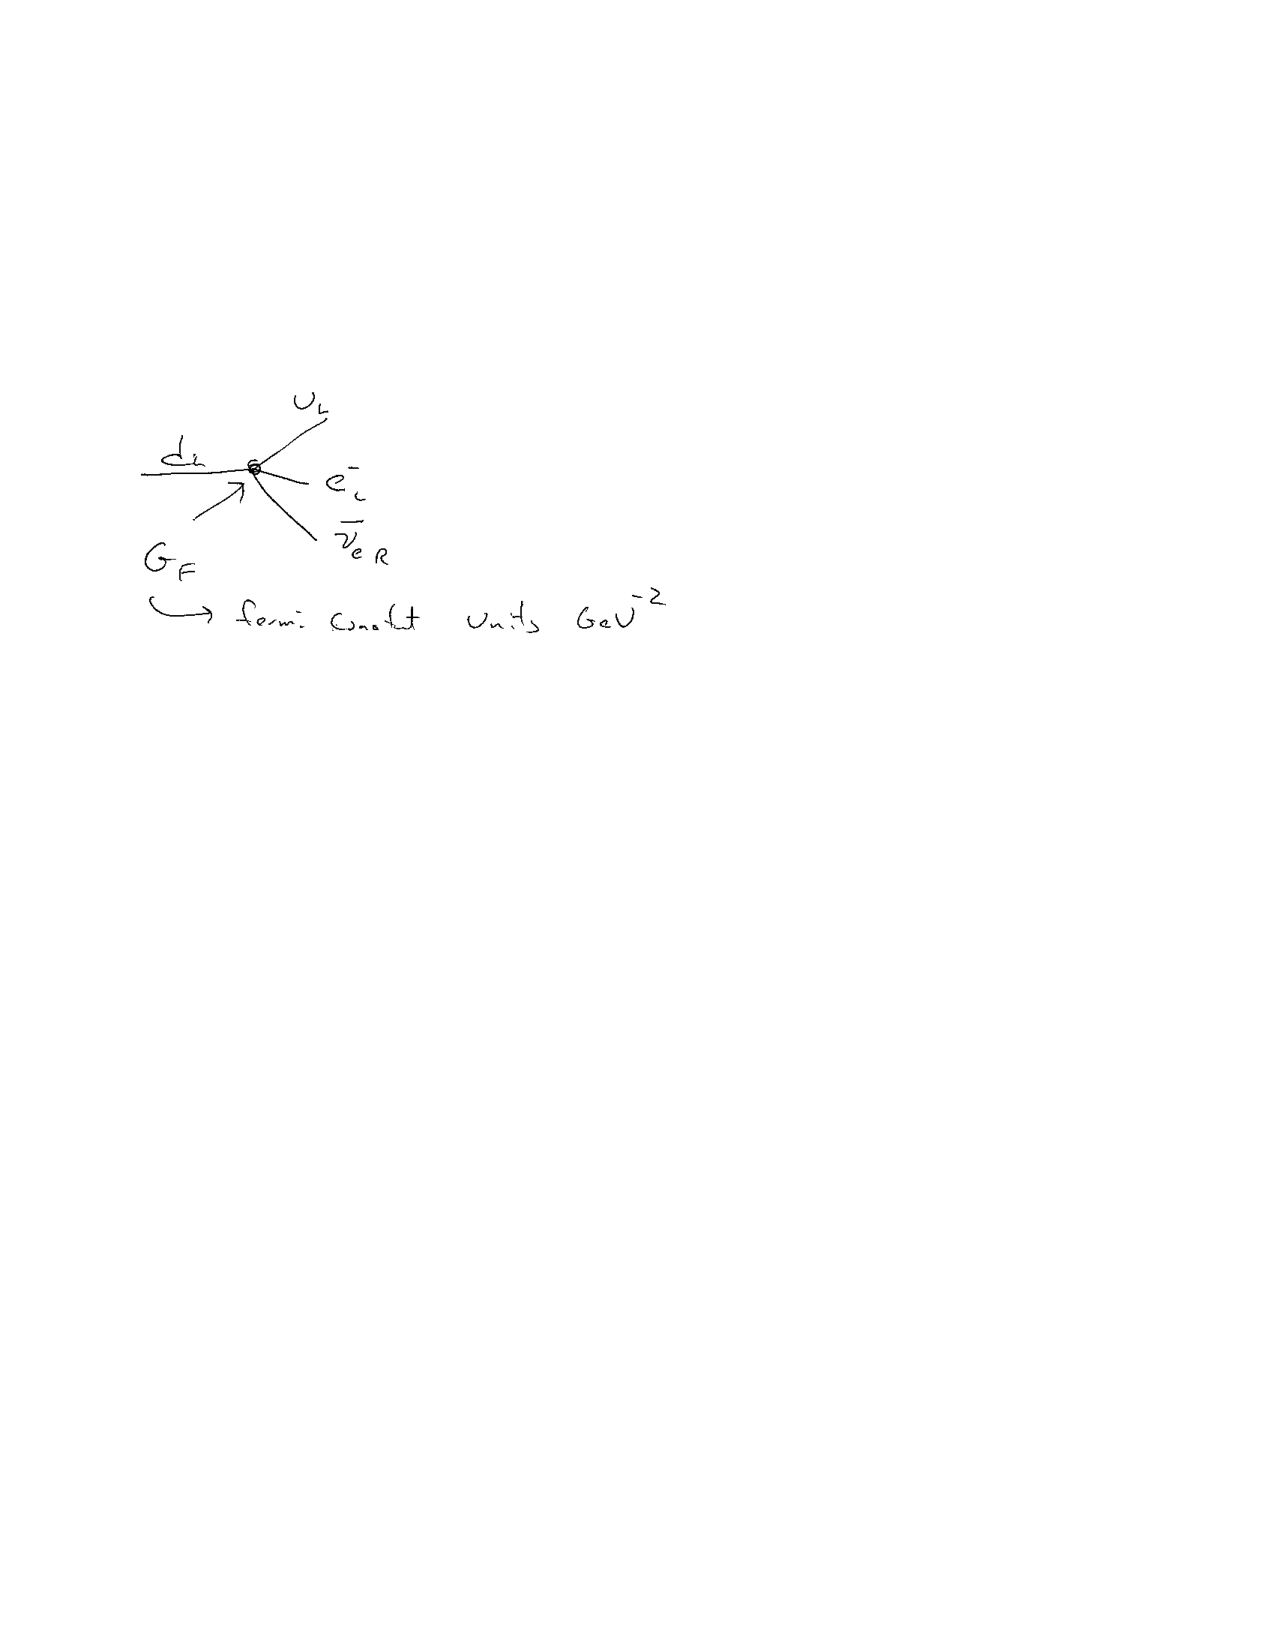
\includegraphics[width=1.0\textwidth]{./BetaDecay.pdf}
\ec
\end{minipage} \hfill
\begin{minipage}{0.4\textwidth}
\be 
L \supset G_F \bar{\nu}_{e_R} e_L d_L u_L
\ee
\end{minipage} \hfill

Also describes the decay of $\mu$s (easier to measure, cleaner to calculate)

\bc
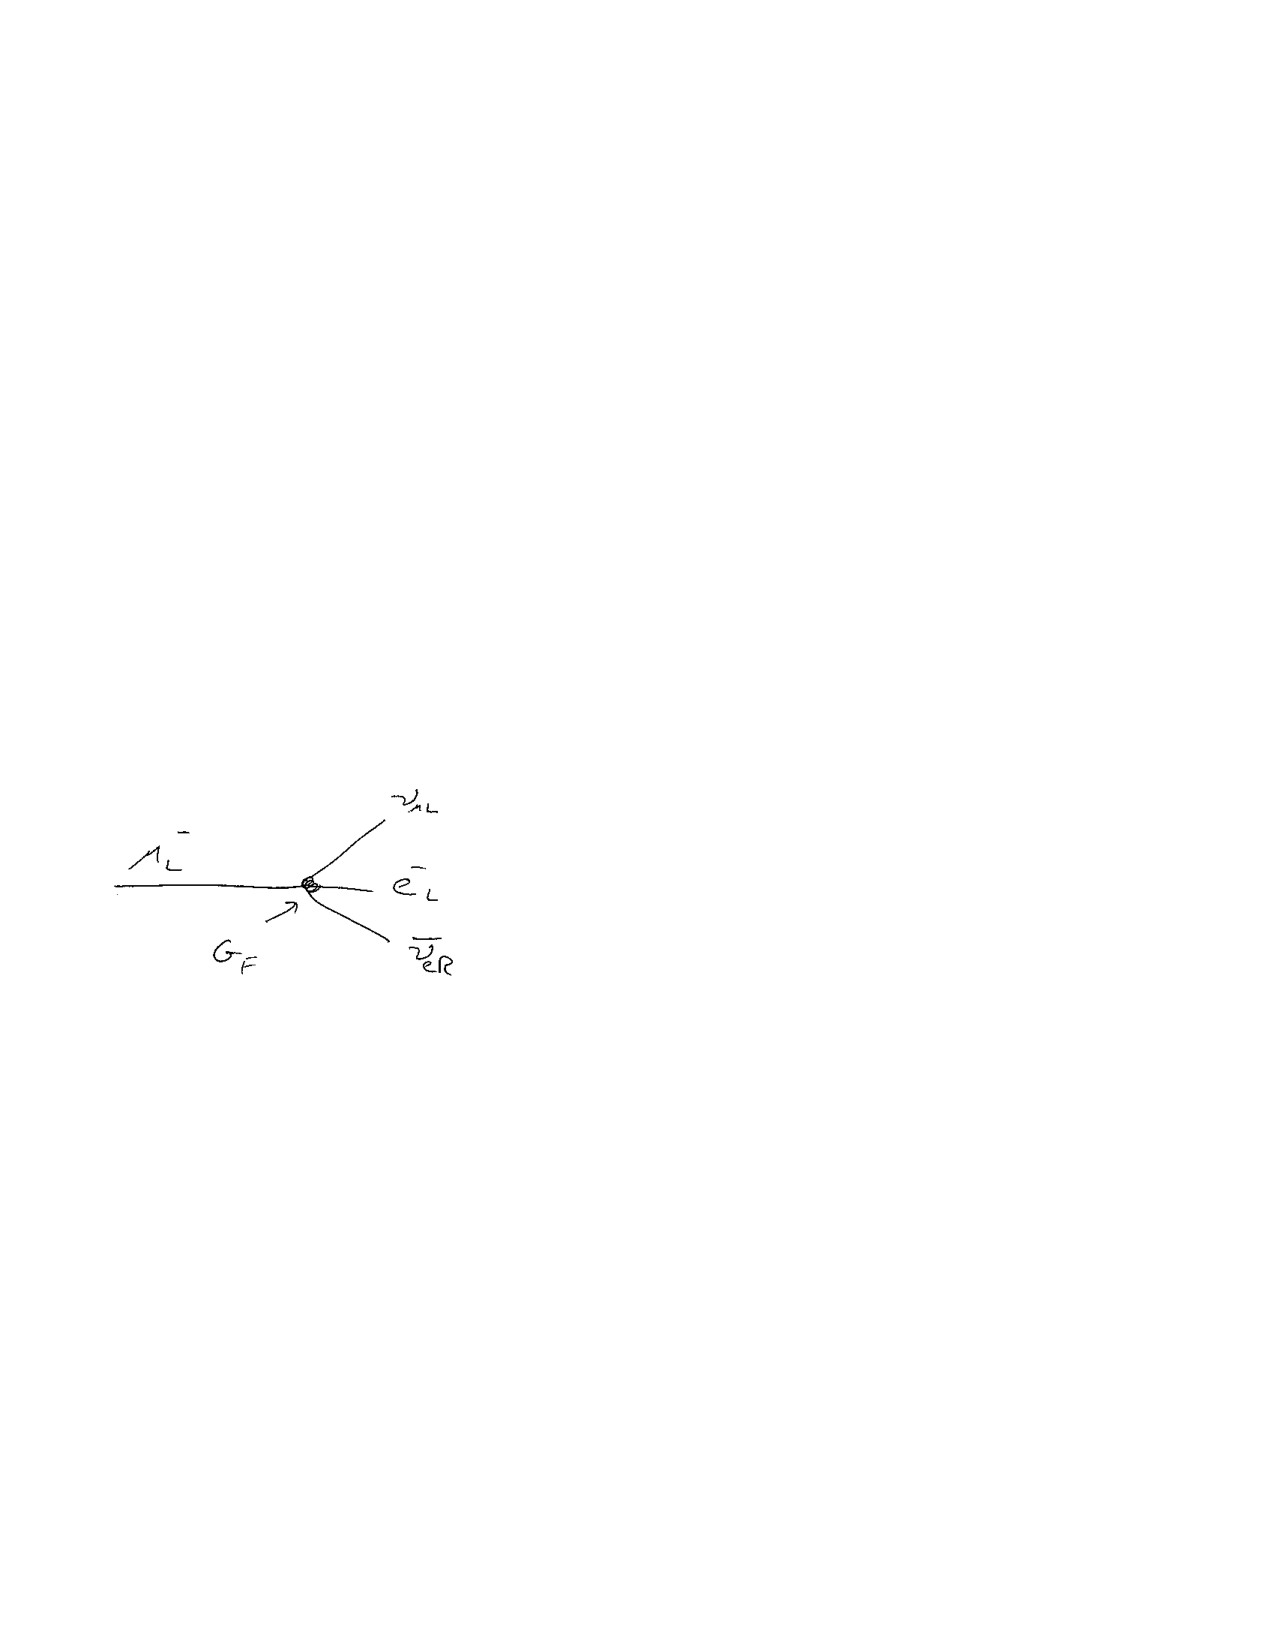
\includegraphics[width=0.5\textwidth]{./MuonDecay.pdf}
\ec

Can apply Feynman rule to Fermi theory and you would get 
\be
\Gamma = \frac{G_F^2 m_\mu^5}{192 \pi^3}
\ee
which is in very good agreement with observations.

However, there are problems built in to this Fermi theory.

Consider cross section to produce $\nu_e$ and $\bar{\nu}_\mu$ from a hypothetical $e\mu$ collider.

\begin{minipage}{0.4\textwidth}
\bc
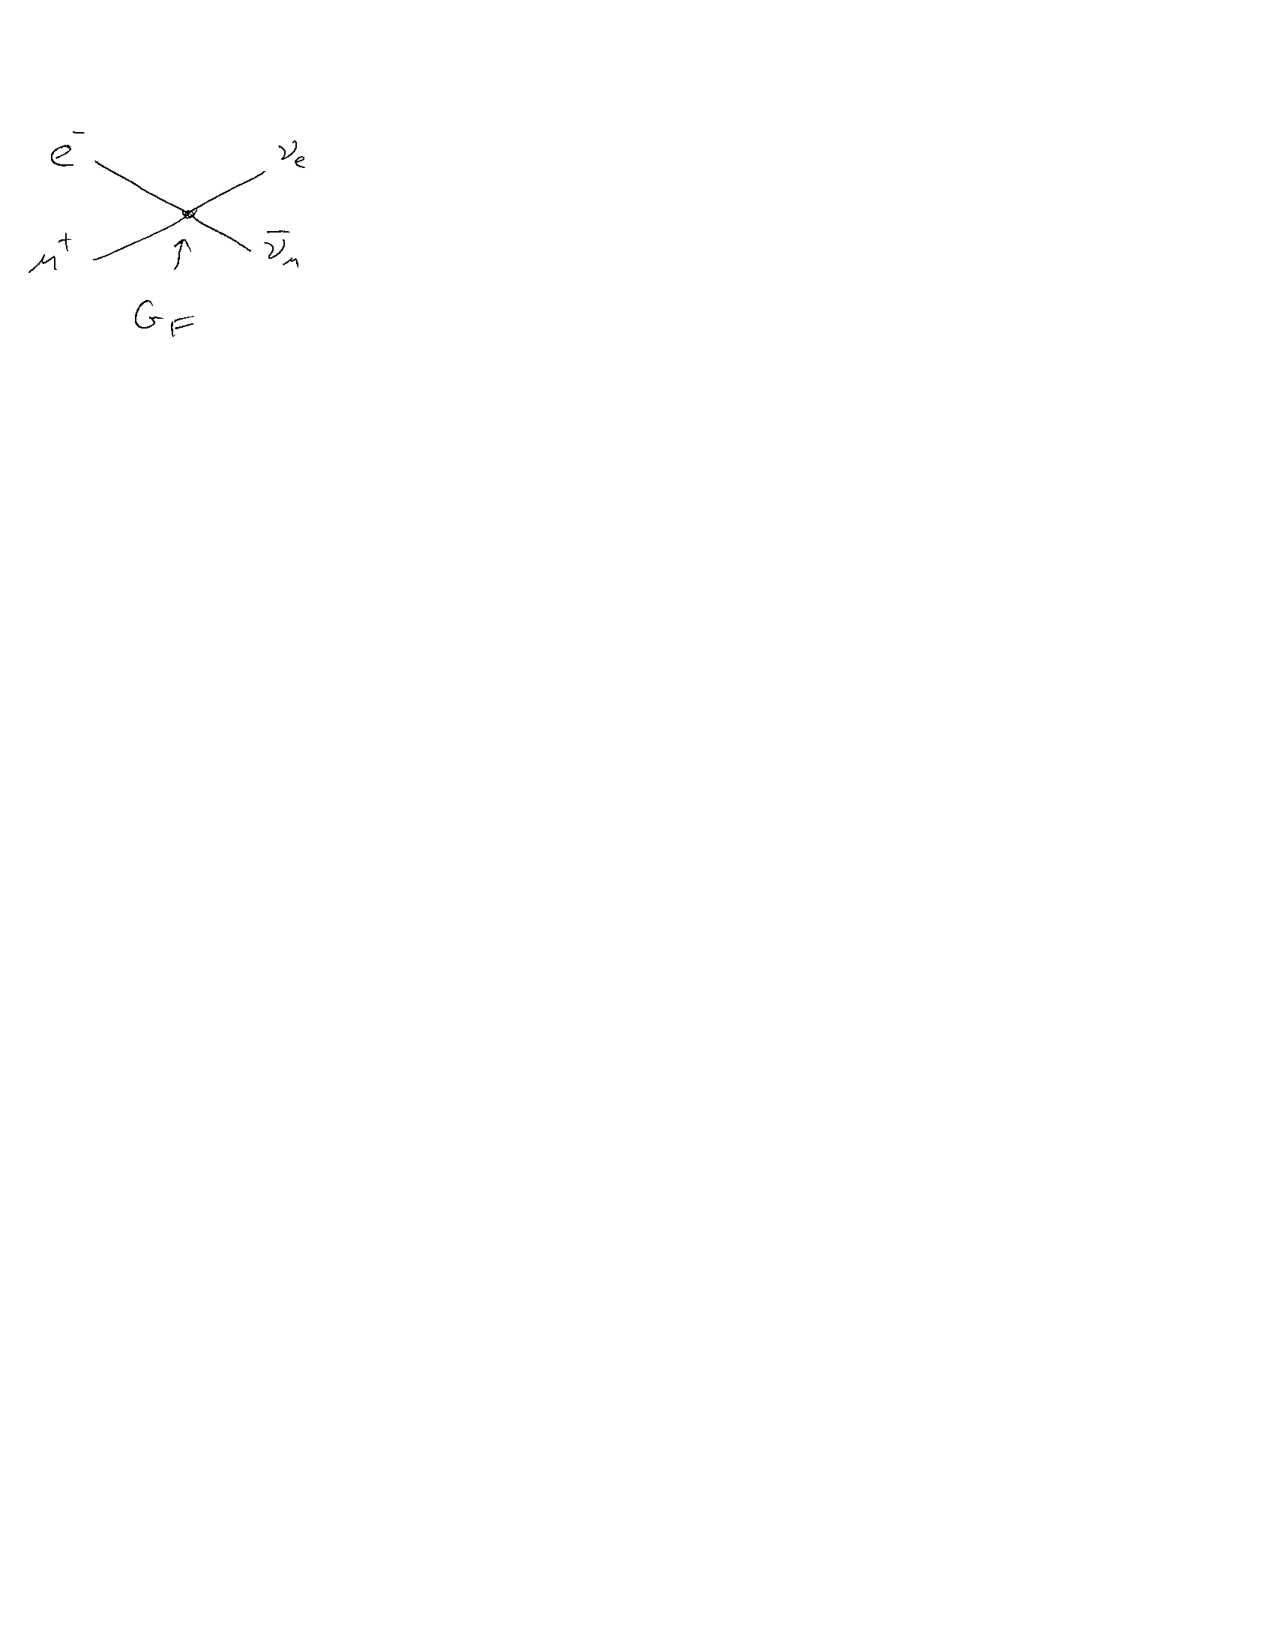
\includegraphics[width=1.0\textwidth]{./emuCollider.pdf}
\ec
\end{minipage} \hfill
\begin{minipage}{0.6\textwidth}
\be
\sigma \sim |M|^2 \sim G_F^2
\ee

\bc
$\sigma$ needs units of Area $\sim \GeV^{-2}$

$\Rightarrow \sigma \sim G_F^2 E_{CM}^2$ 
\ec
\end{minipage}

This is WEIRD, looks like cross section diverges with $E_{CM}$!

Doesn't make physical sense (e and $\mu$ wavelengths shrink with E)

$\sigma$ should get \underline{smaller}!


eg: saw exactly this in $ee\rightarrow \mu\mu$ collisions

\be
\sigma(ee \rightarrow \mu\mu) \sim \frac{1}{E_{CM}^2}
\ee


\lineacross

\underline{Force Carriers}

In QCD and EM effective 4-fermion interactions are controlled by exchange of Boson force carriers (Spin-1)

Assume force carriers associated with weak interaction also Spin-1. 
$G_F$ arises from force carrier exchange, but importantly needs to have the right mass dimension $\Rightarrow$ force carriers of weak interaction must be massive. 

\be
G_F = \frac{1}{m_F^2} \hspace*{1in}  G_F\sim 10^{-5}\ GeV^2   \Rightarrow m_F\sim 300 \GeV
\ee

$m_F$ - ``Fermi Mass''


\underline{\underline{Problematic}} Mass terms for force carriers are not gauge invariant. $m^2A^2$


Leads to Crisis in the field.

}
\end{document}


